\documentclass[tikz,border=8pt]{standalone}
% Shared TikZ style for synorg platform diagrams. Each diagram \input's this
% inside a standalone document. Palette tracks the Material "teal" site theme so
% figures read as one system in light mode (SVGs are theme-neutral otherwise).
\usetikzlibrary{arrows.meta,positioning,shapes.geometric,fit,backgrounds,calc,decorations.pathreplacing}

\definecolor{synteal}{HTML}{00897B}   % primary
\definecolor{synfill}{HTML}{E0F2F1}   % light fill
\definecolor{synamber}{HTML}{B26A00}  % warning / lend
\definecolor{synred}{HTML}{B00020}    % deny / danger
\definecolor{syngrey}{HTML}{5F6368}   % muted

\tikzset{
  >=Stealth,
  font=\sffamily\small,
  box/.style={draw=synteal,line width=0.6pt,rounded corners=2pt,fill=synfill,
              inner sep=5pt,align=center},
  plane/.style={draw=synteal,line width=0.8pt,rounded corners=3pt,fill=synfill,
                inner sep=8pt,align=center},
  state/.style={draw=synteal,line width=0.7pt,circle,fill=synfill,inner sep=3pt,
                minimum size=11mm,align=center,font=\sffamily\footnotesize},
  decision/.style={draw=synteal,line width=0.7pt,diamond,aspect=2,fill=synfill,
                   inner sep=1pt,align=center,font=\sffamily\footnotesize},
  deny/.style={draw=synred,fill=synred!8,text=synred},
  warn/.style={draw=synamber,fill=synamber!10},
  flow/.style={->,line width=0.6pt,draw=syngrey},
  flowlbl/.style={font=\sffamily\footnotesize,text=syngrey,inner sep=2pt},
  note/.style={font=\sffamily\footnotesize\itshape,text=syngrey},
}

\begin{document}
% Staged-reclaim-normal game-day (game-day.md + scenarios.yaml): inference ramps
% to peak while three scheduled waves (05:30/06:00/06:30) drain training borrow
% to zero ahead of the 07:00 ramp; render-start p95 must stay under target across
% the window. Passing this R2 gate is the Phase 2->3 evidence.
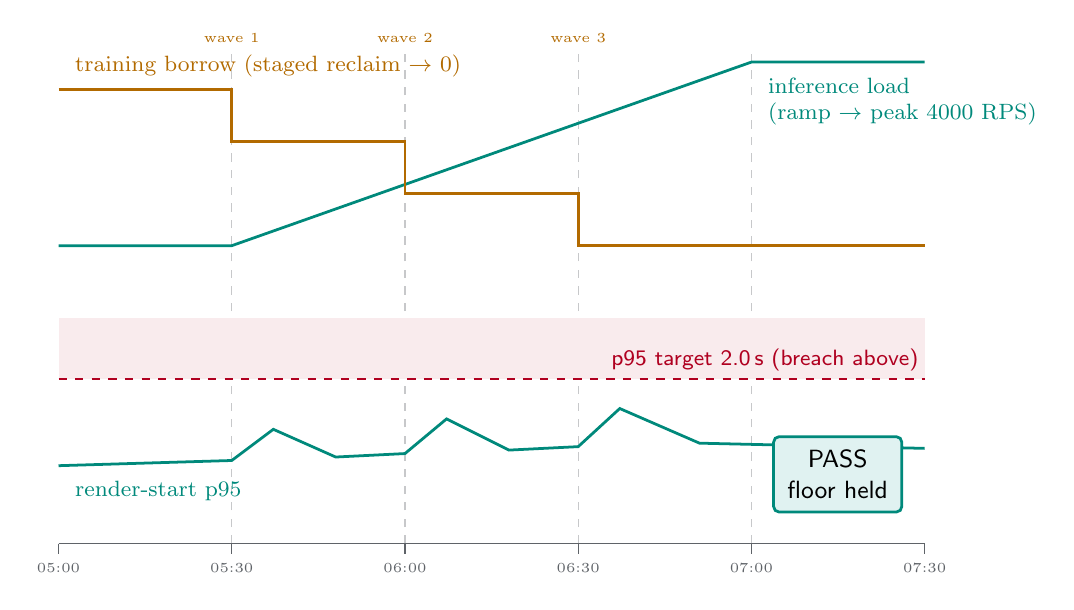
\begin{tikzpicture}[x=44mm,y=22mm]
  % vertical guides at the three waves + ramp, linking both panels
  \foreach \t in {0.5,1.0,1.5,2.0}{
    \draw[syngrey!35,dashed,line width=0.4pt] (\t,0) -- (\t,2.85);
  }

  % ===== top panel: load (y 1.7 .. 2.85) =====
  % inference load ramp
  \draw[line width=1pt,draw=synteal]
    (0,1.72) -- (0.5,1.72) -- (2.0,2.78) -- (2.5,2.78);
  \node[font=\footnotesize,text=synteal,anchor=west,align=left] at (2.02,2.55)
    {inference load\\(ramp $\to$ peak 4000 RPS)};
  % training borrow: staged descending staircase to zero
  \draw[line width=1pt,draw=synamber]
    (0,2.62) -- (0.5,2.62) -- (0.5,2.32) -- (1.0,2.32)
    -- (1.0,2.02) -- (1.5,2.02) -- (1.5,1.72) -- (2.5,1.72);
  \node[font=\footnotesize,text=synamber,anchor=south west] at (0.02,2.64)
    {training borrow (staged reclaim $\to$ 0)};
  % wave markers
  \foreach \t/\n in {0.5/1, 1.0/2, 1.5/3}{
    \node[flowlbl,text=synamber,anchor=south,font=\tiny] at (\t,2.86) {wave \n};
  }

  % ===== bottom panel: render-start p95 (y 0 .. 1.3) =====
  % breach zone above target
  \fill[synred!8] (0,0.95) rectangle (2.5,1.3);
  \draw[dashed,draw=synred,line width=0.6pt] (0,0.95) -- (2.5,0.95);
  \node[flowlbl,text=synred,anchor=south east] at (2.5,0.96) {p95 target 2.0\,s (breach above)};
  % p95 line: small bumps at each wave, never crosses target
  \draw[line width=1pt,draw=synteal]
    (0,0.45) -- (0.5,0.48) -- (0.62,0.66) -- (0.8,0.5)
    -- (1.0,0.52) -- (1.12,0.72) -- (1.3,0.54)
    -- (1.5,0.56) -- (1.62,0.78) -- (1.85,0.58) -- (2.5,0.55);
  \node[font=\footnotesize,text=synteal,anchor=north west] at (0.02,0.42)
    {render-start p95};
  % pass gate
  \node[box,line width=1pt,anchor=west] at (2.06,0.4) {PASS\\floor held};

  % ===== time axis =====
  \draw[draw=syngrey,line width=0.5pt] (0,0) -- (2.5,0);
  \foreach \t/\lbl in {0/05:00, 0.5/05:30, 1.0/06:00, 1.5/06:30, 2.0/07:00, 2.5/07:30}{
    \draw[draw=syngrey] (\t,0) -- (\t,-0.06);
    \node[font=\tiny,text=syngrey,anchor=north] at (\t,-0.06) {\lbl};
  }
\end{tikzpicture}
\end{document}
